\documentclass[12pt,openright,openany,oneside,article,a4paper,brazi]{abntex2}
\usepackage[T1]{fontenc}
\usepackage[utf8]{inputenc}
\usepackage[brazil]{babel}           % estas quatro linhas
\usepackage[alf]{abntex2cite}
%\usepackage[brazil,brazilian]{babel}
\usepackage{lmodern,latexsym,enumerate}
\usepackage{amsmath,amsthm,amsopn,amstext,amscd,amsfonts,amssymb}
\usepackage[dvips]{graphicx}
\usepackage{setspace}
\usepackage{colortbl}
%\usepackage[square,numbers]{natbib}
%\usepackage{natbib}
%\usepackage[loose]{subfigure}
%\usepackage{psfrag}
\usepackage{float}
\usepackage{array} % for defining a new column type
%\usepackage{varwidth}
\usepackage{bm}
\usepackage{url}
\usepackage{indentfirst}
\usepackage{bbding}
\usepackage{pifont}
\usepackage{wasysym}
\usepackage{here,color,xcolor}
%\usepackage{abnt-alf}
%\usepackage[alf]{abntcite}
\usepackage{hyperref}
\usepackage[most]{tcolorbox}
\usepackage{amsmath}


\newcommand\signature[2]{% Nome; funcao
\begin{center}\begin{minipage}{10cm}
    \centering
    \vspace{14pt}\par
    \rule{10cm}{1pt}\par
   \large \textbf{#1}\par
    #2%
\end{minipage}
\end{center}
}


\newcommand\insertdate[1][\today]{
\vfill
\begin{center}
\large #1, \today
\end{center}
}


%\renewcommand{\familydefault}{phv}
\setlrmarginsandblock{2cm}{2cm}{*}
\setulmarginsandblock{2cm}{2cm}{*}
\checkandfixthelayout

\setlength{\ABNTEXcitacaorecuo}{1.8cm}
%configurações do formato do projeto
%\singlespacing Para um espaçamento simples
%\onehalfspacing %Para um espaçamento de 1,5
% \doublespacing Para um espaçamento duplo
\usepackage{times} % times new roman
% pacote babel ou equivalent
%\usepackage[tmargin=2cm,bmargin=2cm,lmargin=2cm,rmargin=2cm]{geometry} % controle das margens 
\setlength{\parindent}{1.3cm}
\setlength{\parskip}{0.2cm} 
\usepackage{titlesec}

\titleformat{\section}[display]
{\large\bfseries}
{\thesection.}{}{}

\newtcolorbox{mybox1}[1]{colback=red!5!white,colframe=red!75!black,fonttitle=\bfseries,title=#1}

\newtcolorbox{mybox}{colback=gray!25,colframe=gray!25, sharp corners=all, height=0.80cm, valign=center}

% Definindo novas cores
\definecolor{verde}{rgb}{0,0.5,0}
% Configurando layout para mostrar codigos C++, R,...
\usepackage{listings}
\lstset{
  language=C++,
  basicstyle=\ttfamily\small,
  keywordstyle=\color{blue},
  stringstyle=\color{verde},
  commentstyle=\color{red},
  extendedchars=true,
  showspaces=false,
  showstringspaces=false,
  numbers=left,
  numberstyle=\tiny,
  breaklines=true,
  backgroundcolor=\color{green!10},
  breakautoindent=true,
  captionpos=b,
  xleftmargin=0pt,
}

\renewcommand{\bibsection}{\section*{Referências}}

\begin{document}

%\pagenumbering{gobble}

\begin{center}


\includegraphics[width=2.17cm,height=2.14cm]{ufcg.png}


{\textbf {UNIVERSIDADE FEDERAL DE CAMPINA GRANDE\\
PRÓ-REITORIA DE PESQUISA E EXTENSÃO\\
COORDENAÇÃO DE PESQUISA}}
\end{center}

 
\vspace{24pt}
\begin{mybox}
\begin{center}
{\Large \textbf{RELATÓRIO DE ATIVIDADES DO ALUNO}}
\end{center}
\end{mybox}
\vspace{12pt}
%%%%%%%%%%%%%%%%%%%%%%%%%%%%%%%%%%%%%%%%%%
%Informações do Projeto
%%%%%%%%%%%%%%%%%%%%%%%%%%%%%%%%%%%%%%%%%%


\begin{flushleft}
{\large \textbf{Programa:} PIVIC}\\
\vspace{14pt}
{\large \textbf{Título do Projeto:} Recuperação da fase de sinais ópticos baseada em machine learning}\\
\vspace{14pt}
{\large \textbf{Aluno:} Silas João Bezerra Soares}\\
\vspace{14pt}
{\large \textbf{Orientador:} Edson Porto da Silva}
\end{flushleft}
\vspace{140pt}

%%%%%%%%%%%%%%%%%%%%%%%%%%%%%%%%%%%%%%
%Informações Assinaturas
%%%%%%%%%%%%%%%%%%%%%%%%%%%%%%%%%%%%%%

\signature{Sr. Silas João Bezerra Soares}{Voluntário}
\signature{Dr. Edson Porto da Silva}{Orientador}

\vspace{5pt}
\insertdate[Campina Grande]


\newpage

%\pagenumbering{gobble}

\section*{Introdução}

Existe uma demanda crescente por redes de comunicações projetadas para atender altas taxas de tráfego,
visto o crescente número de serviços de streaming e dispositivos inteligentes conectados a internet, assim
em algum momento será cada vez mais necessário o uso de tecnologias de comunicação via fibra óptica. Um dos desafios 
dessa área são as transmissões de curta e média distância onde predominam o uso apenas em modulação e detecção da amplitude devido 
ao fato do baixo custo de implementação desses sistemas, porém o mesmo oferece uma capacidade de transmissão 
limitada se comparada aos sistemas coerentes que não só utilizam valores de amplitude como também a fase dos 
sinais que são transmitidos.

Existem inúmeras soluções que estão sendo empregadas no mercado que se utilizam das funcionalidades dos
receptores coerentes combinando a simplicidade dos receptores de detecção direta. O algoritmo de Kramers-Kronig (KK) é 
um exemplo dessas aplicações. Este algoritmo é baseado numa propriedade dos sinais denominada como \textit{sinais de fase mínima}
visando a recuperação de fase, permitindo a reconstrução de um sinal complexo $s(t)$ a partir da medição de sua intensidade 
$\displaystyle\left\lvert s(t)^2 \right\rvert $ utilizando uma sequência de processamento digital de sinais (PDS) baseada nas relações de Kramers-Kronig. 
Atualmente a utilização dos receptores KK fornecem benefícios tanto em desempenho quanto ao consumo de energia. [\citeonline{Mecozzi:16}]  

Assim os principais objetivos desse projeto são obter conhecimentos necessários para a compreensão desses desafios e entendimento introdutório sobre as comunicações ópticas, 
além de conhecer os principais métodos de aprendizagem de máquina utilizando redes neurais artificiais.

\section*{Objetivos}

Durante o período de desenvolvimento da pesquisa, priorizamos o estudo e revisão de disciplinas da graduação que possuam conteúdos relacionados
ao projeto, bem como suprir os requisitos básicos para o entendimento sobre os principais conceitos de sistemas de comunicações ópticas. 
Além do estudo sobre redes neurais artificiais, implementando problemas relacionados a regressão linear e classificação. Logo foram concluídos os seguintes objetivos abaixo: 

  \begin{itemize}
    \item Estudo/revisão bibliográfica sobre redes neurais artificiais.
    \item Estudo/revisão bibliográfica sobre sistemas de comunicações ópticas.
  \end{itemize}

\section*{Material e Métodos/Metodologia}

Para alcançar os objetivos na etapa de estudos sobre sistemas de comunicações ópticas e redes neurais artificiais, foram utilizados os seguintes 
materiais de apoio abaixo. 

  \begin{enumerate}
    \item Aulas fornecidas pela disciplina de comunicações ópticas de forma assíncrona. 
    \item Livro de referência sobre comunicações ópticas. [\citeonline{LightWaveTechnology}]
    \item \hypertarget{label1}{Livro de referência sobre redes neurais artificiais.} [\citeonline{Haykin2009}]
    \item \hypertarget{label2}{Documentação da API do TensorFlow.}
  \end{enumerate}

Nesta primeira etapa adotamos uma metodologia baseada no estudo e implementação de simulações numéricas, para a primeira fase visamos o estudo
de sistemas de comunicações ópticas, como a geração e detecção de sinais ópticos e a realização de simulações númericas apartir do repositório 
fornecido pelo orientador [\citeonline{OpticalCommunications}] e posteriormente o estudo de comunicações coerentes. As próximas etapas se resumiram no estudo e 
implementação de técnicas de aprendizado de máquina associadas a RNAs (redes neurais artificiais) que foram realizados em paralelo com o estudo geral sobre comunicações ópticas.
Neste período foi utilizado os materiais \hyperlink{label1}{3} e \hyperlink{label2}{4} para a implementação de problemas clássicos de machine learning utilizando Python, 
com o auxílio de diversas outras bibliotecas voltadas a computação numérica.

Durante a implementação das soluções baseadas em RNAs vimos como funcionam os neurônios que podem agir como uma unidade de processamento simples, tais neurônios
se unem por meio de conexões sinápticas que formam a base para o projeto de uma grande família de redes neurais artificiais, a importância dos hiperparâmtros (parâmetros ajustáveis que permitem controlar o processo de treinamento do modelo)
de uma rede neural como a definição de uma função de ativação que definem a saída de um neurônio e a importância dessas funções serem diferenciáveis no uso de alguns algoritmos 
como o \textit{Back-Propagation}. Além desses parâmetros podemos definir um otimizador sendo este um dos parâmetros que mais influenciam no 
desempenho da rede neural, o mesmo tem como objetivo diminuir o erro entre os resultados obtidos durante o treinamento em comparação com os resultados desejados. A escolha desses 
parâmetros podem variar de acordo com o problema a ser solucionado, visto que certas funções podem se comportar melhor em uma determinada situação do que outras.  

O próximo passo foi buscar soluções de alguns problemas não lineares como o problema da função XOR, este problema em específico, é bem conhecido na literatura de redes neurais, visto que
um único neurônio clássico não consegue resolver esse obstáculo, assim para resolução do problema optamos pelo uso das redes de múltiplas camadas mais conhecidas como MLP (multilayer perceptron).
Utilizando-se a função de ativação \textit{relu}, obteve-se resultados satisfatórios acertando com precisão as diferentes saídas da função XOR, ao fim do treinamento é possível visualizar as métricas obtidas em forma de gráfico, como a perda e precisão do 
modelo em função das épocas adotadas para o treinamento.

Também foram demonstrados métodos de classificação utilizando um dataset fornecido pelo Keras integrado a própria API do TensorFlow chamado de \textit{fashion-mnist}, neste dataset e possível encontrar 
diferentes peças de roupas e também rótulos empregados para as mesmas. Após o treinamento é possível verificar a saída da rede neural sobre uma predição nas imagens de teste, comparando a imagem devolvida pela RNA com o rótulo da imagem verdadeira. Em seguida é implementado mais um exemplo sobre 
regressão linear tendo como objetivo estimar a inclinação da reta para se adaptar as amostras de dados, sendo modelado por apenas um neurônio, ao final foi possível comparar a equação da reta reproduzida pela RNA 
com a reta produzida por outro algoritmo conhecido como mínimos quadrados. Durante as simulações todos os exemplos se utilizaram do aprendizado supervisionado, além disso foram realizadas avaliações
das métricas que fornecem feedback sobre o desempenho da rede bem como a verificação de eventos como o overfitting. 

Para melhor organização do projeto foi criado um repositório hospedado no GitHub de forma privada, onde acontece o controle de versão sobre os arquivos gerados na pesquisa
onde o orientador pode acompanhar com mais detalhes todo o trabalho que vem sendo realizado.  
 
\section*{Resultados Parciais}

Durante o período de estudos sobre RNAs foi possível adquirir conhecimentos relevantes sobre aprendizagem de máquina, que de certa forma irão ajudar no desenvolvimento da pesquisa. Os resultados obtidos
nesta etapa podem ser visualizados abaixo, como resultados de métricas e previsões efetuadas pelos modelos implementados no TensorFlow. \\

% Imagems dos resultados parciais NN

\begin{figure}[!htb]
  \centering
  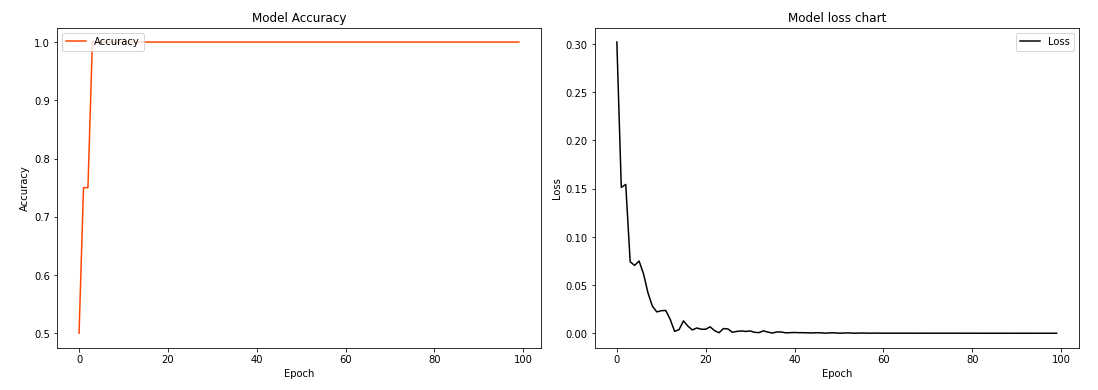
\includegraphics[scale=0.6]{metrics_XOR.PNG}
  \caption{Métricas Obtidas Para o Problema de XOR}
  \label{fig:}
\end{figure}

Com os gráficos acima podemos perceber o baixo índice de perda pela rede neural, bem como a precisão durante o treinamento, logo o modelo proposto para resolução do problema 
foi capaz de lidar com um dos problemas clássicos na literatura de redes neurais.

Abaixo se encontra a resposta da rede neural para os quatro casos possíveis para o problema da função XOR, assim como a arquitetura utilizada na resolução do problema. \\ \\ \\ \\ \\

\begin{figure}[!htb]
  \begin{minipage}[!]{0.55\linewidth}
  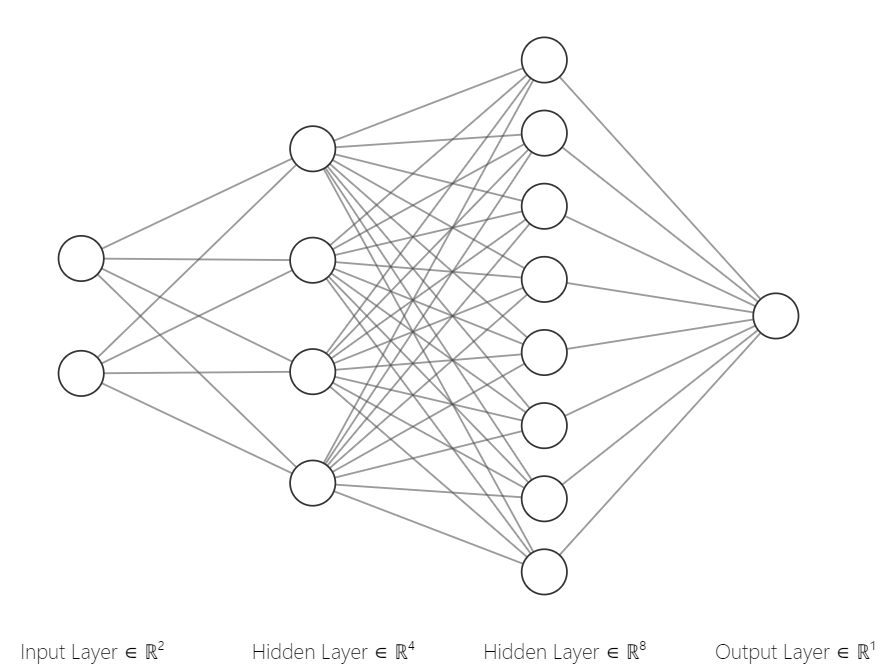
\includegraphics[scale=0.4]{Arquitetura_NN_XOR.PNG}
  \caption{Arquitetura NN}
  \label{fig:}
  \end{minipage}
  \begin{minipage}[!]{0.55\linewidth}
  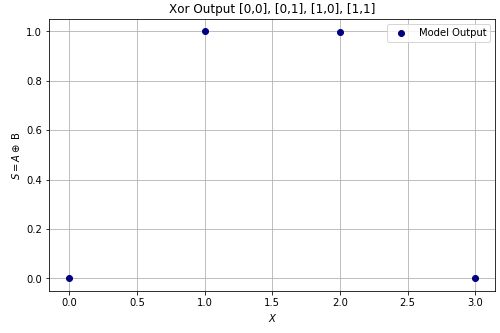
\includegraphics[scale=0.6]{NN_Resposta_Xor.PNG}
  \caption{Resposta do Modelo}
  \label{fig:}
  \end{minipage}
\end{figure}

Para o problema de classificação o dataset possui imagens que correspondem a 28x28 pixels, sendo formado por 60.000 imagens, e da mesma maneira
para os rótulos, para este problema iremos classificar dez imagens diferentes, onde os dez rótulos correspondem a uma matriz de inteiros variando de zero a nove. Abaixo contamos com um conjunto de amostras de dez peças de roupas
diferentes, da mesma forma para os rótulos que foram postos em cada peça de roupa. \\ \\

\begin{figure}[!htb]
  \centering
  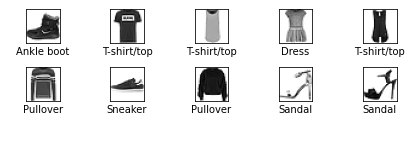
\includegraphics[scale=0.77]{Dataset.PNG}
  \caption{Dataset Fashion-Mnist}
  \label{fig:}
\end{figure}

As métricas obtidas durante o treinamento podem ser visualizadas nas figuras abaixo, como a perda e precisão durante o treinamento, além do mapa de calor associado as classificações feitas pela rede neural. A classificação das 
imagens pela rede neural, se comparadas com os rótulos de testes foram convergentes, atribuindo o mesmo valor presente no vetor de rótulos para a imagem escolhida, isso pode ser visto observando o mapa de calor onde quase todas
as imagens correspondem ao seu devido rótulo verdadeiro.

\begin{figure}[!htb]
  \centering
  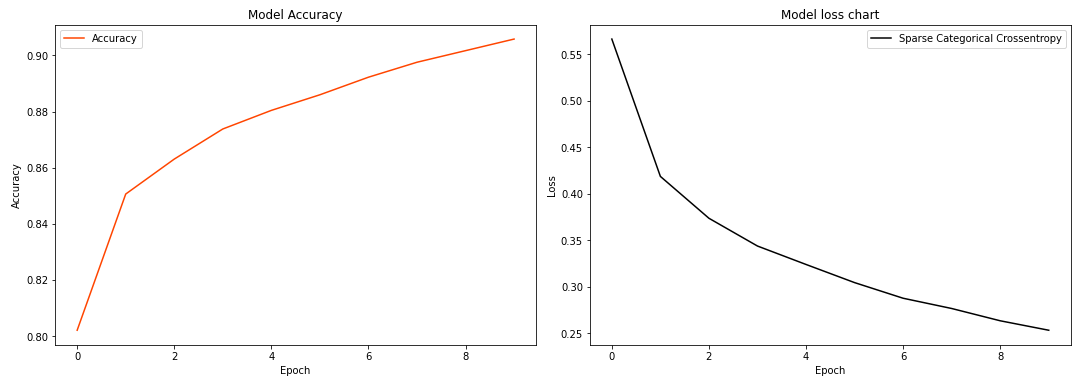
\includegraphics[scale=0.6]{metrics_Classification.PNG}
  \caption{Métricas Obtidas Para o Problema de Classificação}
  \label{fig:}
\end{figure}
\begin{figure}[!htb]
  \centering
  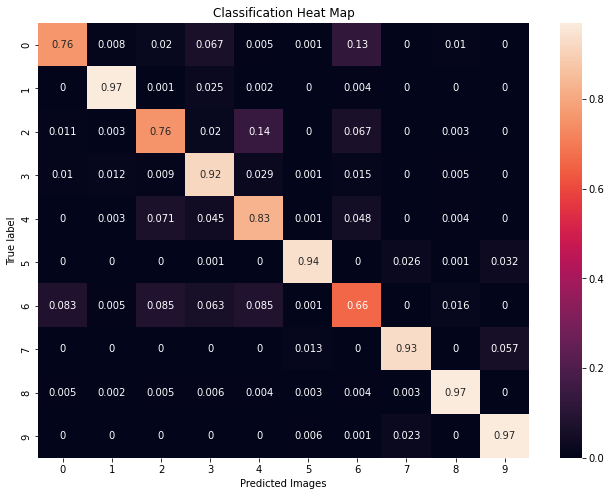
\includegraphics[scale=0.44]{download.png}
  \caption{Heat Map View}
  \label{fig:}
\end{figure}

Desta forma podemos constatar que a rede neural conseguiu realizar as classificações de boa parte das imagens com $\displaystyle 86\%$ de precisão, vale salientar que a rede se utiliza das funções de ativação
relu para camada mais densa composta por 128 neurônios e softmax para camada de saída da rede neural, adotando o Adam como otimizador. \\

Para última implementação foi proposto um modelo com o objetivo de estimar os coeficientes de uma reta que se adéque da melhor forma possível aos dados se utilizando da regressão linear, que é um dos algoritmos fundamentais quando se trata 
de estimar valores ainda desconhecidos de uma determinada variável $\displaystyle y$, dados os valores de algumas outras variáveis $\displaystyle x$, neste problema utilizamos o mesmo princípio. Os dados foram gerados utilizando uma distribuição
aleatória, foi criando um gráfico de dispersão para melhor visualização dos dados como e mostrado na figura 7.

Também foi definido um algoritmo que possui o mesmo objetivo de estimar os coeficientes da reta, utilizando uma técnica de otimização matemática que procura encontrar o 
melhor ajuste possível para um conjunto de dados minimizando a soma dos quadrados das diferenças entre o valor estimado e os dados observados. \\ \\

\begin{figure}[!htb]
  \begin{minipage}[!]{0.48\linewidth}
  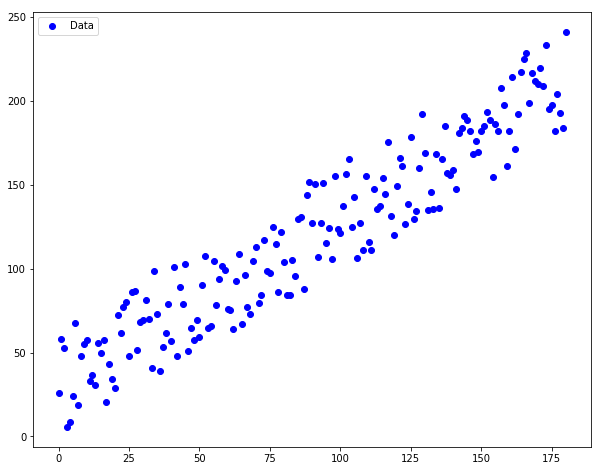
\includegraphics[scale=0.5]{Disperção.PNG}
  \caption{Gráfico de Dispersão}
  \label{fig:}
  \end{minipage}
  \begin{minipage}[!]{0.48\linewidth}
  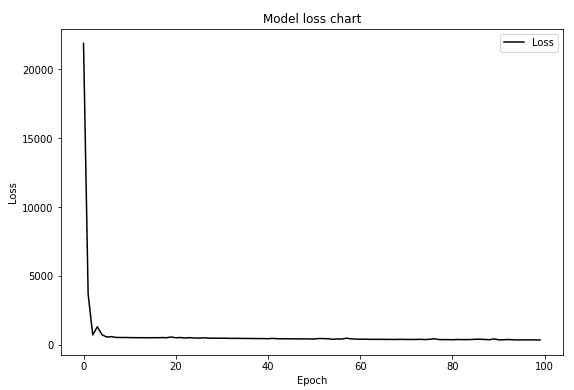
\includegraphics[scale=0.6]{Perda_Regressão.PNG}
  \caption{Perdas Durante o Treinamento}
  \label{fig:}
  \end{minipage}
\end{figure}

Abaixo podemos observar a reta encontrada pela rede neural e também pelo algoritmo de mínimos quadrados. \\

\begin{figure}[!htb]
  \begin{minipage}[!]{0.51\linewidth}
  \begin{center}
    \text{$\displaystyle y_0 = 1.06x + 21.51$}
  \end{center}
  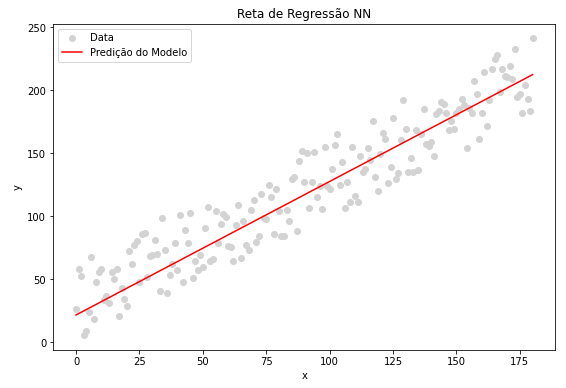
\includegraphics[scale=0.57]{regression_NN.PNG}
  \caption{Resposta do Modelo}
  \label{fig:}
  \end{minipage}
  \begin{minipage}[!]{0.51\linewidth}
  \begin{center}
    \text{$\displaystyle y_1 = 1.00x + 30.13$}
  \end{center}
  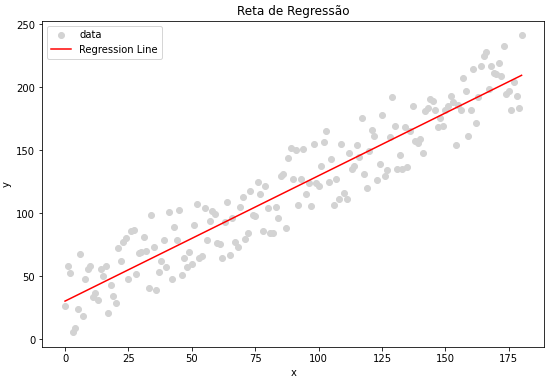
\includegraphics[scale=0.57]{regression_MQ.PNG}
  \caption{Mínimos Quadrados}
  \label{fig:}
  \end{minipage}
\end{figure}

Na figura 11 vemos os resultados finais comparando a reta obtida pelo modelo com a reta obtida por meio do algoritmo de mínimos quadrados. Também é possível vislumbrar que ambos os resultados
estão bem próximos um do outro.

\begin{figure}[!htb]
  \centering
  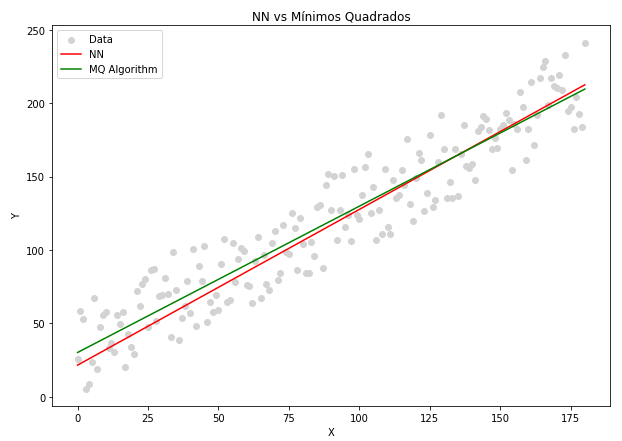
\includegraphics[scale=0.6]{Comparação.PNG}
  \caption{Comparação Entre as Soluções Obtidas}
  \label{fig:}
\end{figure}

Os conhecimentos adquiridos até o momento foram de grande ajuda para dar início ao problema de recuperação de fase implementando modelos sequenciais que se utilizam 
do aprendizado supervisionado, além de validar os modelos que vão ser propostos na resolução do problema. Determinando se RNAs podem ser ferramentas úteis na construção
de algoritmos de PDS para receptores ópticos de baixo custo e alta eficiência energética. \\ \\

Logo podemos constatar que os objetivos iniciais foram satisfeitos, onde foi possível compreender como funcionam os sistemas de comunicações ópticas desde a transmissão até
a detecção dos sinais que incidem sobre o receptor coerente, assim como a compreensão dos parâmetros necessários para realizar as simulações numéricas dos dispositivos que atuam
durante o processo de transmissão e recepção, bem como os fenômenos que ocorrem durante a transmissão na fibra óptica como a dispersão cromática, além de avaliar a qualidade da transmissão
através de métricas como SNR (Relação sinal ruído) e BER (Taxa de erro de bit) e dentre outras, que fazem um papel de extrema importância para definir, tanto o desempenho, como também o custo 
benefício das soluções encontradas.

Por fim os desafios existentes na área de comunicações ópticas, especificamente para algoritmos de recuperação de fase, tem um fator crucial na indústria de telecomunicações, visto que
o desempenho do mesmo combinado com o custo de sua implementação pode possibilitar uma ampla gama de aplicações, principalmente em comunicações de curta e média distância. 

\newpage
%\bibliographystyle{abbrvnat}
\bibliographystyle{abntex2-alf}
\bibliography{ref}
\end{document}